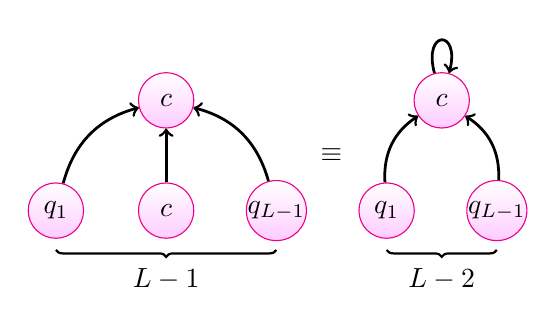
\begin{tikzpicture}[scale=.7]

\tikzset{nodo/.style={circle,minimum size=20pt,inner sep=0pt,draw, top color=white ,bottom color=magenta!20, magenta,text=black}}
\tikzset{label/.style={minimum size=15pt,inner sep=0pt,},}


  \draw (0,0) node[nodo](q1) {$q_1$};
  \draw (2,0) node[nodo](cc) {$c$};
  \draw (4,0) node[nodo](ql) {$q_{L-1}$};
  \draw (2,2) node[nodo](c) {$c$};
\draw[->,line width=1pt] (q1) to[bend left] (c);
\draw[->,line width=1pt] (ql) to[bend right] (c);
\draw[->,line width=1pt] (cc) -- (c);
\draw [thick,decoration={brace,mirror,raise=0.5cm},decorate] (0,0) -- (4,0) ;
\draw (2,-1.25) node[label](c) {$L-1$};

\draw (5,1) node[label](l) {$\equiv$};

  \draw (6,0) node[nodo](q11) {$q_1$};
  \draw (8,0) node[nodo](ql1) {$q_{L-1}$};
  \draw (7,2) node[nodo](c1) {$c$};
\draw[->,line width=1pt] (q11) to[bend left] (c1);
\draw[->,line width=1pt] (ql1) to[bend right] (c1);
\draw[->,line width=1pt] (c1) to [loop above] (c1);
\draw [thick,decoration={brace,mirror,raise=0.5cm},decorate] (6,0) -- (8,0) ;
\draw (7,-1.25) node[label](c) {$L-2$};


\end{tikzpicture}
